% Options for packages loaded elsewhere
\PassOptionsToPackage{unicode}{hyperref}
\PassOptionsToPackage{hyphens}{url}
\PassOptionsToPackage{dvipsnames,svgnames,x11names}{xcolor}
%
\documentclass[
  letterpaper,
  DIV=11,
  numbers=noendperiod]{scrartcl}

\usepackage{amsmath,amssymb}
\usepackage{lmodern}
\usepackage{iftex}
\ifPDFTeX
  \usepackage[T1]{fontenc}
  \usepackage[utf8]{inputenc}
  \usepackage{textcomp} % provide euro and other symbols
\else % if luatex or xetex
  \usepackage{unicode-math}
  \defaultfontfeatures{Scale=MatchLowercase}
  \defaultfontfeatures[\rmfamily]{Ligatures=TeX,Scale=1}
\fi
% Use upquote if available, for straight quotes in verbatim environments
\IfFileExists{upquote.sty}{\usepackage{upquote}}{}
\IfFileExists{microtype.sty}{% use microtype if available
  \usepackage[]{microtype}
  \UseMicrotypeSet[protrusion]{basicmath} % disable protrusion for tt fonts
}{}
\makeatletter
\@ifundefined{KOMAClassName}{% if non-KOMA class
  \IfFileExists{parskip.sty}{%
    \usepackage{parskip}
  }{% else
    \setlength{\parindent}{0pt}
    \setlength{\parskip}{6pt plus 2pt minus 1pt}}
}{% if KOMA class
  \KOMAoptions{parskip=half}}
\makeatother
\usepackage{xcolor}
\setlength{\emergencystretch}{3em} % prevent overfull lines
\setcounter{secnumdepth}{-\maxdimen} % remove section numbering
% Make \paragraph and \subparagraph free-standing
\ifx\paragraph\undefined\else
  \let\oldparagraph\paragraph
  \renewcommand{\paragraph}[1]{\oldparagraph{#1}\mbox{}}
\fi
\ifx\subparagraph\undefined\else
  \let\oldsubparagraph\subparagraph
  \renewcommand{\subparagraph}[1]{\oldsubparagraph{#1}\mbox{}}
\fi

\usepackage{color}
\usepackage{fancyvrb}
\newcommand{\VerbBar}{|}
\newcommand{\VERB}{\Verb[commandchars=\\\{\}]}
\DefineVerbatimEnvironment{Highlighting}{Verbatim}{commandchars=\\\{\}}
% Add ',fontsize=\small' for more characters per line
\usepackage{framed}
\definecolor{shadecolor}{RGB}{241,243,245}
\newenvironment{Shaded}{\begin{snugshade}}{\end{snugshade}}
\newcommand{\AlertTok}[1]{\textcolor[rgb]{0.68,0.00,0.00}{#1}}
\newcommand{\AnnotationTok}[1]{\textcolor[rgb]{0.37,0.37,0.37}{#1}}
\newcommand{\AttributeTok}[1]{\textcolor[rgb]{0.40,0.45,0.13}{#1}}
\newcommand{\BaseNTok}[1]{\textcolor[rgb]{0.68,0.00,0.00}{#1}}
\newcommand{\BuiltInTok}[1]{\textcolor[rgb]{0.00,0.23,0.31}{#1}}
\newcommand{\CharTok}[1]{\textcolor[rgb]{0.13,0.47,0.30}{#1}}
\newcommand{\CommentTok}[1]{\textcolor[rgb]{0.37,0.37,0.37}{#1}}
\newcommand{\CommentVarTok}[1]{\textcolor[rgb]{0.37,0.37,0.37}{\textit{#1}}}
\newcommand{\ConstantTok}[1]{\textcolor[rgb]{0.56,0.35,0.01}{#1}}
\newcommand{\ControlFlowTok}[1]{\textcolor[rgb]{0.00,0.23,0.31}{#1}}
\newcommand{\DataTypeTok}[1]{\textcolor[rgb]{0.68,0.00,0.00}{#1}}
\newcommand{\DecValTok}[1]{\textcolor[rgb]{0.68,0.00,0.00}{#1}}
\newcommand{\DocumentationTok}[1]{\textcolor[rgb]{0.37,0.37,0.37}{\textit{#1}}}
\newcommand{\ErrorTok}[1]{\textcolor[rgb]{0.68,0.00,0.00}{#1}}
\newcommand{\ExtensionTok}[1]{\textcolor[rgb]{0.00,0.23,0.31}{#1}}
\newcommand{\FloatTok}[1]{\textcolor[rgb]{0.68,0.00,0.00}{#1}}
\newcommand{\FunctionTok}[1]{\textcolor[rgb]{0.28,0.35,0.67}{#1}}
\newcommand{\ImportTok}[1]{\textcolor[rgb]{0.00,0.46,0.62}{#1}}
\newcommand{\InformationTok}[1]{\textcolor[rgb]{0.37,0.37,0.37}{#1}}
\newcommand{\KeywordTok}[1]{\textcolor[rgb]{0.00,0.23,0.31}{#1}}
\newcommand{\NormalTok}[1]{\textcolor[rgb]{0.00,0.23,0.31}{#1}}
\newcommand{\OperatorTok}[1]{\textcolor[rgb]{0.37,0.37,0.37}{#1}}
\newcommand{\OtherTok}[1]{\textcolor[rgb]{0.00,0.23,0.31}{#1}}
\newcommand{\PreprocessorTok}[1]{\textcolor[rgb]{0.68,0.00,0.00}{#1}}
\newcommand{\RegionMarkerTok}[1]{\textcolor[rgb]{0.00,0.23,0.31}{#1}}
\newcommand{\SpecialCharTok}[1]{\textcolor[rgb]{0.37,0.37,0.37}{#1}}
\newcommand{\SpecialStringTok}[1]{\textcolor[rgb]{0.13,0.47,0.30}{#1}}
\newcommand{\StringTok}[1]{\textcolor[rgb]{0.13,0.47,0.30}{#1}}
\newcommand{\VariableTok}[1]{\textcolor[rgb]{0.07,0.07,0.07}{#1}}
\newcommand{\VerbatimStringTok}[1]{\textcolor[rgb]{0.13,0.47,0.30}{#1}}
\newcommand{\WarningTok}[1]{\textcolor[rgb]{0.37,0.37,0.37}{\textit{#1}}}

\providecommand{\tightlist}{%
  \setlength{\itemsep}{0pt}\setlength{\parskip}{0pt}}\usepackage{longtable,booktabs,array}
\usepackage{calc} % for calculating minipage widths
% Correct order of tables after \paragraph or \subparagraph
\usepackage{etoolbox}
\makeatletter
\patchcmd\longtable{\par}{\if@noskipsec\mbox{}\fi\par}{}{}
\makeatother
% Allow footnotes in longtable head/foot
\IfFileExists{footnotehyper.sty}{\usepackage{footnotehyper}}{\usepackage{footnote}}
\makesavenoteenv{longtable}
\usepackage{graphicx}
\makeatletter
\def\maxwidth{\ifdim\Gin@nat@width>\linewidth\linewidth\else\Gin@nat@width\fi}
\def\maxheight{\ifdim\Gin@nat@height>\textheight\textheight\else\Gin@nat@height\fi}
\makeatother
% Scale images if necessary, so that they will not overflow the page
% margins by default, and it is still possible to overwrite the defaults
% using explicit options in \includegraphics[width, height, ...]{}
\setkeys{Gin}{width=\maxwidth,height=\maxheight,keepaspectratio}
% Set default figure placement to htbp
\makeatletter
\def\fps@figure{htbp}
\makeatother

\KOMAoption{captions}{tableheading}
\makeatletter
\@ifpackageloaded{tcolorbox}{}{\usepackage[many]{tcolorbox}}
\@ifpackageloaded{fontawesome5}{}{\usepackage{fontawesome5}}
\definecolor{quarto-callout-color}{HTML}{909090}
\definecolor{quarto-callout-note-color}{HTML}{0758E5}
\definecolor{quarto-callout-important-color}{HTML}{CC1914}
\definecolor{quarto-callout-warning-color}{HTML}{EB9113}
\definecolor{quarto-callout-tip-color}{HTML}{00A047}
\definecolor{quarto-callout-caution-color}{HTML}{FC5300}
\definecolor{quarto-callout-color-frame}{HTML}{acacac}
\definecolor{quarto-callout-note-color-frame}{HTML}{4582ec}
\definecolor{quarto-callout-important-color-frame}{HTML}{d9534f}
\definecolor{quarto-callout-warning-color-frame}{HTML}{f0ad4e}
\definecolor{quarto-callout-tip-color-frame}{HTML}{02b875}
\definecolor{quarto-callout-caution-color-frame}{HTML}{fd7e14}
\makeatother
\makeatletter
\makeatother
\makeatletter
\makeatother
\makeatletter
\@ifpackageloaded{caption}{}{\usepackage{caption}}
\AtBeginDocument{%
\ifdefined\contentsname
  \renewcommand*\contentsname{Table of contents}
\else
  \newcommand\contentsname{Table of contents}
\fi
\ifdefined\listfigurename
  \renewcommand*\listfigurename{List of Figures}
\else
  \newcommand\listfigurename{List of Figures}
\fi
\ifdefined\listtablename
  \renewcommand*\listtablename{List of Tables}
\else
  \newcommand\listtablename{List of Tables}
\fi
\ifdefined\figurename
  \renewcommand*\figurename{Figure}
\else
  \newcommand\figurename{Figure}
\fi
\ifdefined\tablename
  \renewcommand*\tablename{Table}
\else
  \newcommand\tablename{Table}
\fi
}
\@ifpackageloaded{float}{}{\usepackage{float}}
\floatstyle{ruled}
\@ifundefined{c@chapter}{\newfloat{codelisting}{h}{lop}}{\newfloat{codelisting}{h}{lop}[chapter]}
\floatname{codelisting}{Listing}
\newcommand*\listoflistings{\listof{codelisting}{List of Listings}}
\makeatother
\makeatletter
\@ifpackageloaded{caption}{}{\usepackage{caption}}
\@ifpackageloaded{subcaption}{}{\usepackage{subcaption}}
\makeatother
\makeatletter
\@ifpackageloaded{tcolorbox}{}{\usepackage[many]{tcolorbox}}
\makeatother
\makeatletter
\@ifundefined{shadecolor}{\definecolor{shadecolor}{rgb}{.97, .97, .97}}
\makeatother
\makeatletter
\makeatother
\ifLuaTeX
  \usepackage{selnolig}  % disable illegal ligatures
\fi
\IfFileExists{bookmark.sty}{\usepackage{bookmark}}{\usepackage{hyperref}}
\IfFileExists{xurl.sty}{\usepackage{xurl}}{} % add URL line breaks if available
\urlstyle{same} % disable monospaced font for URLs
\hypersetup{
  pdftitle={Homework 4},
  pdfauthor={Gaurang Kakade},
  colorlinks=true,
  linkcolor={blue},
  filecolor={Maroon},
  citecolor={Blue},
  urlcolor={Blue},
  pdfcreator={LaTeX via pandoc}}

\title{Homework 4}
\author{{Gaurang Kakade}}
\date{}

\begin{document}
\maketitle
\ifdefined\Shaded\renewenvironment{Shaded}{\begin{tcolorbox}[interior hidden, borderline west={3pt}{0pt}{shadecolor}, frame hidden, breakable, enhanced, sharp corners, boxrule=0pt]}{\end{tcolorbox}}\fi

\renewcommand*\contentsname{Table of contents}
{
\hypersetup{linkcolor=}
\setcounter{tocdepth}{3}
\tableofcontents
}
\href{https://github.com/psu-stat380/hw-4}{Link to the Github
repository}

\begin{center}\rule{0.5\linewidth}{0.5pt}\end{center}

\begin{tcolorbox}[enhanced jigsaw, breakable, colframe=quarto-callout-important-color-frame, bottomtitle=1mm, leftrule=.75mm, bottomrule=.15mm, arc=.35mm, titlerule=0mm, coltitle=black, colback=white, colbacktitle=quarto-callout-important-color!10!white, opacitybacktitle=0.6, toptitle=1mm, opacityback=0, title=\textcolor{quarto-callout-important-color}{\faExclamation}\hspace{0.5em}{Due: Sun, Apr 2, 2023 @ 11:59pm}, toprule=.15mm, left=2mm, rightrule=.15mm]

Please read the instructions carefully before submitting your
assignment.

\begin{enumerate}
\def\labelenumi{\arabic{enumi}.}
\tightlist
\item
  This assignment requires you to only upload a \texttt{PDF} file on
  Canvas
\item
  Don't collapse any code cells before submitting.
\item
  Remember to make sure all your code output is rendered properly before
  uploading your submission.
\end{enumerate}

⚠️ Please add your name to the author information in the frontmatter
before submitting your assignment ⚠️

\end{tcolorbox}

We will be using the following libraries:

\begin{Shaded}
\begin{Highlighting}[]
\NormalTok{packages }\OtherTok{\textless{}{-}} \FunctionTok{c}\NormalTok{(}
  \StringTok{"dplyr"}\NormalTok{, }
  \StringTok{"readr"}\NormalTok{, }
  \StringTok{"tidyr"}\NormalTok{, }
  \StringTok{"purrr"}\NormalTok{, }
  \StringTok{"stringr"}\NormalTok{, }
  \StringTok{"corrplot"}\NormalTok{, }
  \StringTok{"car"}\NormalTok{, }
  \StringTok{"caret"}\NormalTok{, }
  \StringTok{"torch"}\NormalTok{, }
  \StringTok{"nnet"}\NormalTok{, }
  \StringTok{"broom"}
\NormalTok{)}

\CommentTok{\# renv::install(packages)}
\FunctionTok{sapply}\NormalTok{(packages, require, }\AttributeTok{character.only=}\NormalTok{T)}
\end{Highlighting}
\end{Shaded}

\begin{verbatim}
Loading required package: dplyr
\end{verbatim}

\begin{verbatim}

Attaching package: 'dplyr'
\end{verbatim}

\begin{verbatim}
The following objects are masked from 'package:stats':

    filter, lag
\end{verbatim}

\begin{verbatim}
The following objects are masked from 'package:base':

    intersect, setdiff, setequal, union
\end{verbatim}

\begin{verbatim}
Loading required package: readr
\end{verbatim}

\begin{verbatim}
Loading required package: tidyr
\end{verbatim}

\begin{verbatim}
Loading required package: purrr
\end{verbatim}

\begin{verbatim}
Loading required package: stringr
\end{verbatim}

\begin{verbatim}
Loading required package: corrplot
\end{verbatim}

\begin{verbatim}
corrplot 0.92 loaded
\end{verbatim}

\begin{verbatim}
Loading required package: car
\end{verbatim}

\begin{verbatim}
Loading required package: carData
\end{verbatim}

\begin{verbatim}

Attaching package: 'car'
\end{verbatim}

\begin{verbatim}
The following object is masked from 'package:purrr':

    some
\end{verbatim}

\begin{verbatim}
The following object is masked from 'package:dplyr':

    recode
\end{verbatim}

\begin{verbatim}
Loading required package: caret
\end{verbatim}

\begin{verbatim}
Loading required package: ggplot2
\end{verbatim}

\begin{verbatim}
Loading required package: lattice
\end{verbatim}

\begin{verbatim}

Attaching package: 'caret'
\end{verbatim}

\begin{verbatim}
The following object is masked from 'package:purrr':

    lift
\end{verbatim}

\begin{verbatim}
Loading required package: torch
\end{verbatim}

\begin{verbatim}
Loading required package: nnet
\end{verbatim}

\begin{verbatim}
Loading required package: broom
\end{verbatim}

\begin{verbatim}
   dplyr    readr    tidyr    purrr  stringr corrplot      car    caret 
    TRUE     TRUE     TRUE     TRUE     TRUE     TRUE     TRUE     TRUE 
   torch     nnet    broom 
    TRUE     TRUE     TRUE 
\end{verbatim}

\hypertarget{section}{%
\subsection{\texorpdfstring{}{    }}\label{section}}

\hypertarget{question-1}{%
\subsection{Question 1}\label{question-1}}

\begin{tcolorbox}[enhanced jigsaw, breakable, colframe=quarto-callout-tip-color-frame, bottomtitle=1mm, leftrule=.75mm, bottomrule=.15mm, arc=.35mm, titlerule=0mm, coltitle=black, colback=white, colbacktitle=quarto-callout-tip-color!10!white, opacitybacktitle=0.6, toptitle=1mm, opacityback=0, title=\textcolor{quarto-callout-tip-color}{\faLightbulb}\hspace{0.5em}{30 points}, toprule=.15mm, left=2mm, rightrule=.15mm]

Automatic differentiation using \texttt{torch}

\end{tcolorbox}

1.1 (5 points)

Consider \(g(x, y)\) given by \[
g(x, y) = (x - 3)^2 + (y - 4)^2.
\]

Using elementary calculus derive the expressions for

\[
\frac{d}{dx}g(x, y), \quad \text{and} \quad \frac{d}{dy}g(x, y).
\]

Using your answer from above, what is the answer to \[
\frac{d}{dx}g(x, y) \Bigg|_{(x=3, y=4)} \quad \text{and} \quad \frac{d}{dy}g(x, y) \Bigg|_{(x=3, y=4)} ?
\]

Define \(g(x, y)\) as a function in R, compute the gradient of
\(g(x, y)\) with respect to \(x=3\) and \(y=4\). Does the answer match
what you expected?

\begin{Shaded}
\begin{Highlighting}[]
\CommentTok{\# Defining the function g(x,y)}
\NormalTok{g }\OtherTok{\textless{}{-}} \ControlFlowTok{function}\NormalTok{(x,y)\{}
  \FunctionTok{return}\NormalTok{((x[}\DecValTok{1}\NormalTok{] }\SpecialCharTok{{-}} \DecValTok{3}\NormalTok{)}\SpecialCharTok{\^{}}\DecValTok{2} \SpecialCharTok{+}\NormalTok{ (x[}\DecValTok{2}\NormalTok{] }\SpecialCharTok{{-}} \DecValTok{4}\NormalTok{)}\SpecialCharTok{\^{}}\DecValTok{2}\NormalTok{)}
\NormalTok{\}}
\CommentTok{\# Computing the gradient of g(x,y) at x = 3 and y = 4}
\FunctionTok{library}\NormalTok{(numDeriv)}
\NormalTok{grad\_g}\OtherTok{\textless{}{-}}\FunctionTok{grad}\NormalTok{(g, }\FunctionTok{c}\NormalTok{(}\DecValTok{3}\NormalTok{,}\DecValTok{4}\NormalTok{))}
\NormalTok{grad\_g}
\end{Highlighting}
\end{Shaded}

\begin{verbatim}
[1] 0 0
\end{verbatim}

\begin{center}\rule{0.5\linewidth}{0.5pt}\end{center}

1.2 (10 points)

\[\newcommand{\u}{\boldsymbol{u}}\newcommand{\v}{\boldsymbol{v}}\]

Consider \(h(\u, \v)\) given by \[
h(\u, \v) = (\u \cdot \v)^3,
\] where \(\u \cdot \v\) denotes the dot product of two vectors, i.e.,
\(\u \cdot \v = \sum_{i=1}^n u_i v_i.\)

Using elementary calculus derive the expressions for the gradients

\[
\begin{aligned}
\nabla_\u h(\u, \v) &= \Bigg(\frac{d}{du_1}h(\u, \v), \frac{d}{du_2}h(\u, \v), \dots, \frac{d}{du_n}h(\u, \v)\Bigg)
\end{aligned}
\]

Using your answer from above, what is the answer to
\(\nabla_\u h(\u, \v)\) when \(n=10\) and

\[
\begin{aligned}
\u = (-1, +1, -1, +1, -1, +1, -1, +1, -1, +1)\\
\v = (-1, -1, -1, -1, -1, +1, +1, +1, +1, +1)
\end{aligned}
\]

Define \(h(\u, \v)\) as a function in R, initialize the two vectors
\(\u\) and \(\v\) as \texttt{torch\_tensor}s. Compute the gradient of
\(h(\u, \v)\) with respect to \(\u\). Does the answer match what you
expected?

\begin{Shaded}
\begin{Highlighting}[]
\FunctionTok{library}\NormalTok{(torch)}

\NormalTok{u }\OtherTok{\textless{}{-}} \FunctionTok{torch\_tensor}\NormalTok{(}\FunctionTok{c}\NormalTok{(}\SpecialCharTok{{-}}\DecValTok{1}\NormalTok{,}\DecValTok{1}\NormalTok{,}\SpecialCharTok{{-}}\DecValTok{1}\NormalTok{,}\DecValTok{1}\NormalTok{,}\SpecialCharTok{{-}}\DecValTok{1}\NormalTok{,}\DecValTok{1}\NormalTok{,}\SpecialCharTok{{-}}\DecValTok{1}\NormalTok{,}\DecValTok{1}\NormalTok{,}\SpecialCharTok{{-}}\DecValTok{1}\NormalTok{,}\DecValTok{1}\NormalTok{), }\AttributeTok{requires\_grad =} \ConstantTok{TRUE}\NormalTok{)}
\NormalTok{v }\OtherTok{\textless{}{-}} \FunctionTok{torch\_tensor}\NormalTok{(}\FunctionTok{c}\NormalTok{(}\SpecialCharTok{{-}}\DecValTok{1}\NormalTok{,}\SpecialCharTok{{-}}\DecValTok{1}\NormalTok{,}\SpecialCharTok{{-}}\DecValTok{1}\NormalTok{,}\SpecialCharTok{{-}}\DecValTok{1}\NormalTok{,}\SpecialCharTok{{-}}\DecValTok{1}\NormalTok{,}\DecValTok{1}\NormalTok{,}\DecValTok{1}\NormalTok{,}\DecValTok{1}\NormalTok{,}\DecValTok{1}\NormalTok{,}\DecValTok{1}\NormalTok{), }\AttributeTok{requires\_grad =} \ConstantTok{TRUE}\NormalTok{)}

\NormalTok{h }\OtherTok{\textless{}{-}} \ControlFlowTok{function}\NormalTok{(u,v)\{}
\NormalTok{  (}\FunctionTok{torch\_dot}\NormalTok{(u,v)}\SpecialCharTok{\^{}}\DecValTok{3}\NormalTok{)}
\NormalTok{\}}

\NormalTok{h\_uv }\OtherTok{\textless{}{-}} \FunctionTok{h}\NormalTok{(u, v)}
\NormalTok{h\_uv}\SpecialCharTok{$}\FunctionTok{backward}\NormalTok{()}
\NormalTok{u}\SpecialCharTok{$}\NormalTok{grad}
\end{Highlighting}
\end{Shaded}

\begin{verbatim}
torch_tensor
-12
-12
-12
-12
-12
 12
 12
 12
 12
 12
[ CPUFloatType{10} ]
\end{verbatim}

\begin{center}\rule{0.5\linewidth}{0.5pt}\end{center}

Yes, the result is in line with my expectations.

1.3 (5 points)

Consider the following function \[
f(z) = z^4 - 6z^2 - 3z + 4
\]

Derive the expression for \[
f'(z_0) = \frac{df}{dz}\Bigg|_{z=z_0}
\] and evaluate \(f'(z_0)\) when \(z_0 = -3.5\).

Define \(f(z)\) as a function in R, and using the \texttt{torch} library
compute \(f'(-3.5)\).

\begin{Shaded}
\begin{Highlighting}[]
\FunctionTok{library}\NormalTok{(torch)}
\NormalTok{f }\OtherTok{\textless{}{-}} \ControlFlowTok{function}\NormalTok{(z)\{}
  \FunctionTok{return}\NormalTok{(z}\SpecialCharTok{\^{}}\DecValTok{4} \SpecialCharTok{{-}} \DecValTok{6}\SpecialCharTok{*}\NormalTok{z}\SpecialCharTok{\^{}}\DecValTok{2} \SpecialCharTok{{-}} \DecValTok{3}\SpecialCharTok{*}\NormalTok{z }\SpecialCharTok{+} \DecValTok{4}\NormalTok{)}
\NormalTok{\}}

\NormalTok{z\_0 }\OtherTok{\textless{}{-}} \FunctionTok{torch\_tensor}\NormalTok{(}\SpecialCharTok{{-}}\FloatTok{3.5}\NormalTok{, }\AttributeTok{requires\_grad =} \ConstantTok{TRUE}\NormalTok{)}
\NormalTok{y }\OtherTok{\textless{}{-}} \FunctionTok{f}\NormalTok{(z\_0)}

\NormalTok{y}\SpecialCharTok{$}\FunctionTok{backward}\NormalTok{()}
\NormalTok{z\_0}\SpecialCharTok{$}\NormalTok{grad}
\end{Highlighting}
\end{Shaded}

\begin{verbatim}
torch_tensor
-132.5000
[ CPUFloatType{1} ]
\end{verbatim}

\begin{center}\rule{0.5\linewidth}{0.5pt}\end{center}

1.4 (5 points)

For the same function \(f\), initialize \(z[1] = -3.5\), and perform
\(n=100\) iterations of \textbf{gradient descent}, i.e.,

\begin{quote}
\$z{[}\{k+1\}{]} = z{[}k{]} - \textbackslash eta f'(z{[}k{]})
\textbackslash{} \textbackslash{} \textbackslash{} \textbackslash{} \$
for \(k = 1, 2, \dots, 100\)
\end{quote}

Plot the curve \(f\) and add taking \(\eta = 0.02\), add the points
\(\{z_0, z_1, z_2, \dots z_{100}\}\) obtained using gradient descent to
the plot. What do you observe?

\begin{center}\rule{0.5\linewidth}{0.5pt}\end{center}

\begin{Shaded}
\begin{Highlighting}[]
\NormalTok{n }\OtherTok{\textless{}{-}} \DecValTok{100}
\NormalTok{z }\OtherTok{\textless{}{-}} \SpecialCharTok{{-}}\FloatTok{3.5}
\NormalTok{eta }\OtherTok{\textless{}{-}} \FloatTok{0.02}
\NormalTok{z\_values }\OtherTok{\textless{}{-}} \FunctionTok{c}\NormalTok{(z)}

\ControlFlowTok{for}\NormalTok{(i }\ControlFlowTok{in} \DecValTok{1}\SpecialCharTok{:}\NormalTok{n)\{}
\NormalTok{  df }\OtherTok{\textless{}{-}} \DecValTok{4} \SpecialCharTok{*}\NormalTok{ z }\SpecialCharTok{\^{}} \DecValTok{3} \SpecialCharTok{{-}} \DecValTok{12} \SpecialCharTok{*}\NormalTok{ z }\SpecialCharTok{{-}} \DecValTok{3}
\NormalTok{  z }\OtherTok{\textless{}{-}}\NormalTok{ z }\SpecialCharTok{{-}}\NormalTok{ eta }\SpecialCharTok{*}\NormalTok{ df}
  
\NormalTok{  z\_values }\OtherTok{\textless{}{-}} \FunctionTok{c}\NormalTok{(z\_values, }\DecValTok{2}\NormalTok{)}
\NormalTok{\}}

\CommentTok{\# plotting the curve}
\NormalTok{x\_values }\OtherTok{\textless{}{-}} \FunctionTok{seq}\NormalTok{(}\SpecialCharTok{{-}}\DecValTok{4}\NormalTok{,}\DecValTok{4}\NormalTok{, }\AttributeTok{by =} \FloatTok{0.01}\NormalTok{)}
\NormalTok{y\_values }\OtherTok{\textless{}{-}} \FunctionTok{f}\NormalTok{(x\_values)}

\NormalTok{df\_f }\OtherTok{\textless{}{-}} \FunctionTok{data.frame}\NormalTok{(}\AttributeTok{x =}\NormalTok{ x\_values, }\AttributeTok{y =}\NormalTok{ y\_values)}
\NormalTok{df\_z }\OtherTok{\textless{}{-}} \FunctionTok{data.frame}\NormalTok{(}\AttributeTok{x =}\NormalTok{ z\_values, }\AttributeTok{y =} \FunctionTok{f}\NormalTok{(z\_values))}

\FunctionTok{ggplot}\NormalTok{() }\SpecialCharTok{+} 
  \FunctionTok{geom\_line}\NormalTok{(}\AttributeTok{data =}\NormalTok{ df\_f, }\FunctionTok{aes}\NormalTok{(x,y), }\AttributeTok{color =} \StringTok{"lightblue"}\NormalTok{,    }\AttributeTok{size =} \DecValTok{1}\NormalTok{) }\SpecialCharTok{+} 
  \FunctionTok{geom\_point}\NormalTok{(}\AttributeTok{data =}\NormalTok{ df\_z, }\FunctionTok{aes}\NormalTok{(x,y), }\AttributeTok{color =} \StringTok{"maroon"}\NormalTok{,      }\AttributeTok{size =} \DecValTok{3}\NormalTok{) }\SpecialCharTok{+} 
  \FunctionTok{ggtitle}\NormalTok{(}\StringTok{"Gradient Descent for f(z)"}\NormalTok{) }\SpecialCharTok{+} 
  \FunctionTok{ylab}\NormalTok{(}\StringTok{"z"}\NormalTok{) }\SpecialCharTok{+} 
  \FunctionTok{xlab}\NormalTok{(}\StringTok{"f(z)"}\NormalTok{)}
\end{Highlighting}
\end{Shaded}

\begin{verbatim}
Warning: Using `size` aesthetic for lines was deprecated in ggplot2 3.4.0.
i Please use `linewidth` instead.
\end{verbatim}

\begin{figure}[H]

{\centering 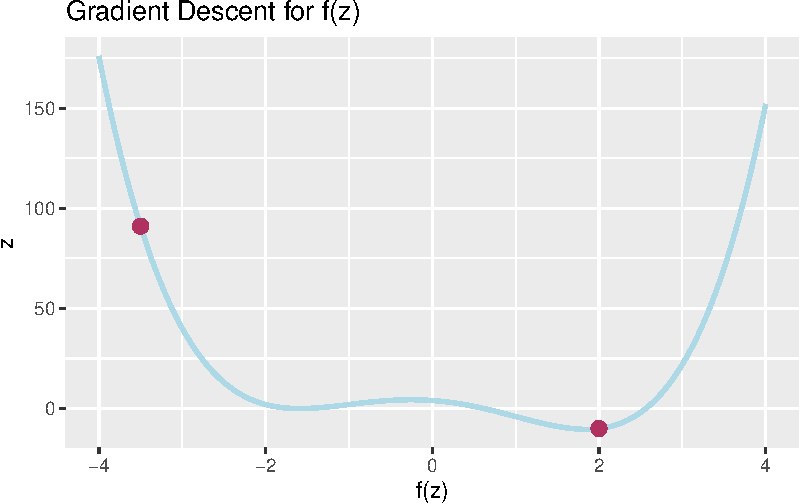
\includegraphics{index_files/figure-pdf/unnamed-chunk-5-1.pdf}

}

\end{figure}

\begin{quote}
The gradient descent algorithm for the function is depicted in the graph
that was produced. The gradient descent algorithm's iterative results
are shown by the maroon dots, while the light blue line depicts the
curve of the function f(z) and its values are represented by the light
blue line. The value of z increases while the algorithm runs, moving
closer to the function's minimum at z not equal to 0.522. The maroon
dots represent the z values that were determined after each algorithm
iteration, and we can see that they converge to the minimal value.
\end{quote}

1.5 (5 points)

Redo the same analysis as \textbf{Question 1.4}, but this time using
\(\eta = 0.03\). What do you observe? What can you conclude from this
analysis

\begin{Shaded}
\begin{Highlighting}[]
\NormalTok{n }\OtherTok{\textless{}{-}} \DecValTok{100}
\NormalTok{z }\OtherTok{\textless{}{-}} \SpecialCharTok{{-}}\FloatTok{3.5}
\NormalTok{eta }\OtherTok{\textless{}{-}} \FloatTok{0.03}
\NormalTok{z\_values }\OtherTok{\textless{}{-}} \FunctionTok{c}\NormalTok{(z)}

\ControlFlowTok{for}\NormalTok{(i }\ControlFlowTok{in} \DecValTok{1}\SpecialCharTok{:}\NormalTok{n)\{}
\NormalTok{  df }\OtherTok{\textless{}{-}} \DecValTok{4} \SpecialCharTok{*}\NormalTok{ z }\SpecialCharTok{\^{}} \DecValTok{3} \SpecialCharTok{{-}} \DecValTok{12} \SpecialCharTok{*}\NormalTok{ z }\SpecialCharTok{{-}} \DecValTok{3}
\NormalTok{  z }\OtherTok{\textless{}{-}}\NormalTok{ z }\SpecialCharTok{{-}}\NormalTok{ eta }\SpecialCharTok{*}\NormalTok{ df}
  
\NormalTok{  z\_values }\OtherTok{\textless{}{-}} \FunctionTok{c}\NormalTok{(z\_values, }\DecValTok{2}\NormalTok{)}
\NormalTok{\}}

\CommentTok{\# plotting the curve}
\NormalTok{x\_values }\OtherTok{\textless{}{-}} \FunctionTok{seq}\NormalTok{(}\SpecialCharTok{{-}}\DecValTok{4}\NormalTok{,}\DecValTok{4}\NormalTok{, }\AttributeTok{by =} \FloatTok{0.01}\NormalTok{)}
\NormalTok{y\_values }\OtherTok{\textless{}{-}} \FunctionTok{f}\NormalTok{(x\_values)}

\NormalTok{df\_f }\OtherTok{\textless{}{-}} \FunctionTok{data.frame}\NormalTok{(}\AttributeTok{x =}\NormalTok{ x\_values, }\AttributeTok{y =}\NormalTok{ y\_values)}
\NormalTok{df\_z }\OtherTok{\textless{}{-}} \FunctionTok{data.frame}\NormalTok{(}\AttributeTok{x =}\NormalTok{ z\_values, }\AttributeTok{y =} \FunctionTok{f}\NormalTok{(z\_values))}

\FunctionTok{ggplot}\NormalTok{() }\SpecialCharTok{+} 
  \FunctionTok{geom\_line}\NormalTok{(}\AttributeTok{data =}\NormalTok{ df\_f, }\FunctionTok{aes}\NormalTok{(x,y), }\AttributeTok{color =} \StringTok{"lightblue"}\NormalTok{,    }\AttributeTok{size =} \DecValTok{1}\NormalTok{) }\SpecialCharTok{+} 
  \FunctionTok{geom\_point}\NormalTok{(}\AttributeTok{data =}\NormalTok{ df\_z, }\FunctionTok{aes}\NormalTok{(x,y), }\AttributeTok{color =} \StringTok{"maroon"}\NormalTok{,      }\AttributeTok{size =} \DecValTok{3}\NormalTok{) }\SpecialCharTok{+} 
  \FunctionTok{ggtitle}\NormalTok{(}\StringTok{"Gradient Descent for f(z)"}\NormalTok{) }\SpecialCharTok{+} 
  \FunctionTok{ylab}\NormalTok{(}\StringTok{"z"}\NormalTok{) }\SpecialCharTok{+} 
  \FunctionTok{xlab}\NormalTok{(}\StringTok{"f(z)"}\NormalTok{)}
\end{Highlighting}
\end{Shaded}

\begin{figure}[H]

{\centering 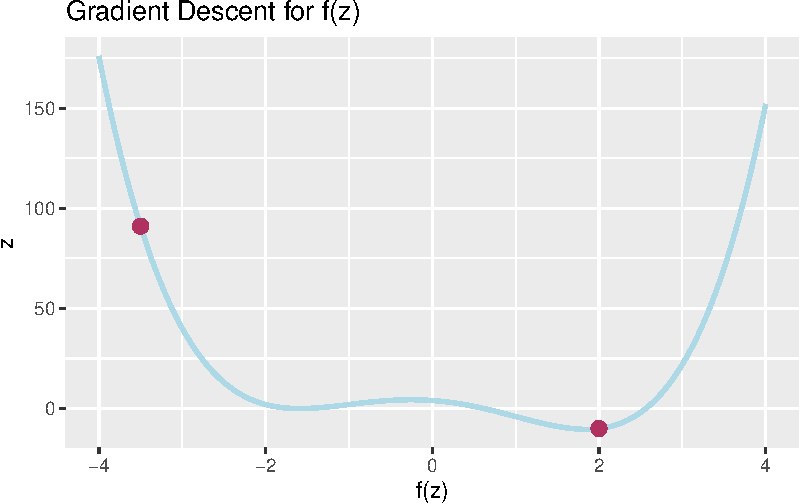
\includegraphics{index_files/figure-pdf/unnamed-chunk-6-1.pdf}

}

\end{figure}

\begin{quote}
The gradient descent algorithm for the function is depicted in the graph
that was produced. The gradient descent algorithm's iterative results
are shown by the maroon dots, while the light blue line depicts the
curve of the function f(z) and its values are represented by the light
blue line. The value of z increases while the algorithm runs, moving
closer to the function's minimum at z not equal to 0.522. The maroon
dots represent the z values that were determined after each algorithm
iteration, and we can see that they converge to the minimal value.

Due to a higher eta value, the path chosen is a little different from
the previous graph in that the marron dots oscillate before convergeing
on the minimum (0.03 instead of 0.02). We can observe from the analysis
that the gradient descent algorithm's performance depends on the
learning rate that is selected. Slower convergence is the result of a
lower learning rate, while overshooting and oscillation around the
minimum are the results of a higher learning rate. We can draw the
conclusion that it's critical to pick a learning pace that's appropriate
for the particular issue being tackled.
\end{quote}

---

\hypertarget{question-2}{%
\subsection{Question 2}\label{question-2}}

\begin{tcolorbox}[enhanced jigsaw, breakable, colframe=quarto-callout-tip-color-frame, bottomtitle=1mm, leftrule=.75mm, bottomrule=.15mm, arc=.35mm, titlerule=0mm, coltitle=black, colback=white, colbacktitle=quarto-callout-tip-color!10!white, opacitybacktitle=0.6, toptitle=1mm, opacityback=0, title=\textcolor{quarto-callout-tip-color}{\faLightbulb}\hspace{0.5em}{50 points}, toprule=.15mm, left=2mm, rightrule=.15mm]

Logistic regression and interpretation of effect sizes

\end{tcolorbox}

For this question we will use the \textbf{Titanic} dataset from the
Stanford data archive. This dataset contains information about
passengers aboard the Titanic and whether or not they survived.

\begin{center}\rule{0.5\linewidth}{0.5pt}\end{center}

2.1 (5 points)

Read the data from the following URL as a tibble in R. Preprocess the
data such that the variables are of the right data type, e.g., binary
variables are encoded as factors, and convert all column names to lower
case for consistency. Let's also rename the response variable
\texttt{Survival} to \texttt{y} for convenience.

\begin{Shaded}
\begin{Highlighting}[]
\NormalTok{url }\OtherTok{\textless{}{-}} \StringTok{"https://web.stanford.edu/class/archive/cs/cs109/cs109.1166/stuff/titanic.csv"}

\NormalTok{df }\OtherTok{\textless{}{-}} \FunctionTok{read.csv}\NormalTok{(url) }\SpecialCharTok{\%\textgreater{}\%}
  \FunctionTok{drop\_na}\NormalTok{()}
\CommentTok{\# Converting binary variables to factors. Pclass is a categorical variable, but it we can convert it to a factor.  }
\NormalTok{df }\OtherTok{\textless{}{-}}\NormalTok{ df }\SpecialCharTok{\%\textgreater{}\%}
  \FunctionTok{mutate}\NormalTok{(}\AttributeTok{Sex =} \FunctionTok{as.factor}\NormalTok{(Sex),}
         \AttributeTok{Survived =} \FunctionTok{as.factor}\NormalTok{(Survived))}

\CommentTok{\# Converting all the columns names to lower case for consistency. }
\FunctionTok{colnames}\NormalTok{(df) }\OtherTok{\textless{}{-}} \FunctionTok{tolower}\NormalTok{(}\FunctionTok{colnames}\NormalTok{(df))}

\CommentTok{\# Renaming the response variable \textasciigrave{}Survival\textasciigrave{} to \textasciigrave{}y\textasciigrave{} for convenience. }
\NormalTok{df }\OtherTok{\textless{}{-}}\NormalTok{ df}\SpecialCharTok{\%\textgreater{}\%}
  \FunctionTok{rename}\NormalTok{(}\AttributeTok{y =}\NormalTok{ survived)}
\end{Highlighting}
\end{Shaded}

\begin{center}\rule{0.5\linewidth}{0.5pt}\end{center}

2.2 (5 points)

Visualize the correlation matrix of all numeric columns in \texttt{df}
using \texttt{corrplot()}

\begin{Shaded}
\begin{Highlighting}[]
\NormalTok{cor\_matrix }\OtherTok{\textless{}{-}}\NormalTok{ df }\SpecialCharTok{\%\textgreater{}\%} 
  \FunctionTok{keep}\NormalTok{(is.numeric) }\SpecialCharTok{\%\textgreater{}\%}
  \FunctionTok{cor}\NormalTok{()}
\FunctionTok{corrplot}\NormalTok{(cor\_matrix,}\AttributeTok{type =} \StringTok{"upper"}\NormalTok{, }\AttributeTok{order =} \StringTok{"hclust"}\NormalTok{ )}
\end{Highlighting}
\end{Shaded}

\begin{figure}[H]

{\centering 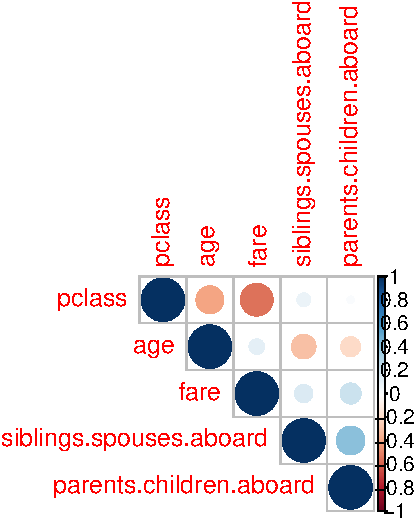
\includegraphics{index_files/figure-pdf/unnamed-chunk-8-1.pdf}

}

\end{figure}

\begin{center}\rule{0.5\linewidth}{0.5pt}\end{center}

2.3 (10 points)

Fit a logistic regression model to predict the probability of surviving
the titanic as a function of:

\begin{itemize}
\tightlist
\item
  \texttt{pclass}
\item
  \texttt{sex}
\item
  \texttt{age}
\item
  \texttt{fare}
\item
  \texttt{\#\ siblings}
\item
  \texttt{\#\ parents}
\end{itemize}

\begin{Shaded}
\begin{Highlighting}[]
\NormalTok{full\_model }\OtherTok{\textless{}{-}} \FunctionTok{glm}\NormalTok{(y }\SpecialCharTok{\textasciitilde{}}\NormalTok{ pclass }\SpecialCharTok{+}\NormalTok{ sex }\SpecialCharTok{+}\NormalTok{ age }\SpecialCharTok{+}\NormalTok{ fare  }\SpecialCharTok{+}\NormalTok{ siblings.spouses.aboard }\SpecialCharTok{+}\NormalTok{ parents.children.aboard, df, }\AttributeTok{family =} \FunctionTok{binomial}\NormalTok{())}
\FunctionTok{summary}\NormalTok{(full\_model)}
\end{Highlighting}
\end{Shaded}

\begin{verbatim}

Call:
glm(formula = y ~ pclass + sex + age + fare + siblings.spouses.aboard + 
    parents.children.aboard, family = binomial(), data = df)

Deviance Residuals: 
    Min       1Q   Median       3Q      Max  
-2.7789  -0.5976  -0.3987   0.6156   2.4409  

Coefficients:
                         Estimate Std. Error z value Pr(>|z|)    
(Intercept)              5.297252   0.557409   9.503  < 2e-16 ***
pclass                  -1.177659   0.146079  -8.062 7.52e-16 ***
sexmale                 -2.757282   0.200416 -13.758  < 2e-16 ***
age                     -0.043474   0.007723  -5.629 1.81e-08 ***
fare                     0.002786   0.002389   1.166 0.243680    
siblings.spouses.aboard -0.401831   0.110712  -3.630 0.000284 ***
parents.children.aboard -0.106505   0.118588  -0.898 0.369127    
---
Signif. codes:  0 '***' 0.001 '**' 0.01 '*' 0.05 '.' 0.1 ' ' 1

(Dispersion parameter for binomial family taken to be 1)

    Null deviance: 1182.77  on 886  degrees of freedom
Residual deviance:  780.93  on 880  degrees of freedom
AIC: 794.93

Number of Fisher Scoring iterations: 5
\end{verbatim}

\begin{center}\rule{0.5\linewidth}{0.5pt}\end{center}

2.4 (30 points)

Provide an interpretation for the slope and intercept terms estimated in
\texttt{full\_model} in terms of the log-odds of survival in the titanic
and in terms of the odds-ratio (if the covariate is also categorical).

The log-odds of survival are the intercept (5.297252), which is the
value when all other variables are set to zero. Due to the fact that it
is a constant element in the model, it cannot be simply interpreted in
terms of survival probability. This coefficient, pclass (-1.177659),
shows how the log-odds of survival alter with each increase in class
level (from 1st to 2nd class or from 2nd to 3rd class). According to
chances ratios, exp(-1.177659) 0.308, which indicates that the
probability of surviving drop by roughly 69.2\% for every level of
class.

\begin{tcolorbox}[enhanced jigsaw, breakable, colframe=quarto-callout-color-frame, bottomtitle=1mm, leftrule=.75mm, bottomrule=.15mm, arc=.35mm, titlerule=0mm, coltitle=black, colback=white, colbacktitle=quarto-callout-color!10!white, opacitybacktitle=0.6, toptitle=1mm, opacityback=0, title={}, toprule=.15mm, left=2mm, rightrule=.15mm]

Recall the definition of logistic regression from the lecture notes, and
also recall how we interpreted the slope in the linear regression model
(particularly when the covariate was categorical).

\end{tcolorbox}

---

\hypertarget{question-3}{%
\subsection{Question 3}\label{question-3}}

\begin{tcolorbox}[enhanced jigsaw, breakable, colframe=quarto-callout-tip-color-frame, bottomtitle=1mm, leftrule=.75mm, bottomrule=.15mm, arc=.35mm, titlerule=0mm, coltitle=black, colback=white, colbacktitle=quarto-callout-tip-color!10!white, opacitybacktitle=0.6, toptitle=1mm, opacityback=0, title=\textcolor{quarto-callout-tip-color}{\faLightbulb}\hspace{0.5em}{70 points}, toprule=.15mm, left=2mm, rightrule=.15mm]

Variable selection and logistic regression in \texttt{torch}

\end{tcolorbox}

\begin{center}\rule{0.5\linewidth}{0.5pt}\end{center}

3.1 (15 points)

Complete the following function \texttt{overview} which takes in two
categorical vectors (\texttt{predicted} and \texttt{expected}) and
outputs:

\begin{itemize}
\tightlist
\item
  The prediction accuracy
\item
  The prediction error
\item
  The false positive rate, and
\item
  The false negative rate
\end{itemize}

\begin{Shaded}
\begin{Highlighting}[]
\NormalTok{overview }\OtherTok{\textless{}{-}} \ControlFlowTok{function}\NormalTok{(predicted, expected)\{}
\NormalTok{    total\_false\_positives }\OtherTok{\textless{}{-}} \FunctionTok{sum}\NormalTok{(predicted }\SpecialCharTok{!=}\NormalTok{expected }\SpecialCharTok{\&}\NormalTok{ predicted }\SpecialCharTok{==} \DecValTok{1}\NormalTok{)}
\NormalTok{    total\_true\_positives }\OtherTok{\textless{}{-}} \FunctionTok{sum}\NormalTok{(predicted }\SpecialCharTok{==}\NormalTok{ expected }\SpecialCharTok{\&}\NormalTok{ expected }\SpecialCharTok{==} \DecValTok{1}\NormalTok{)}
\NormalTok{    total\_false\_negatives }\OtherTok{\textless{}{-}} \FunctionTok{sum}\NormalTok{(predicted }\SpecialCharTok{!=}\NormalTok{ expected }\SpecialCharTok{\&}\NormalTok{ predicted }\SpecialCharTok{==} \DecValTok{0}\NormalTok{)}
\NormalTok{    total\_true\_negatives }\OtherTok{\textless{}{-}} \FunctionTok{sum}\NormalTok{(predicted }\SpecialCharTok{==}\NormalTok{ expected }\SpecialCharTok{\&}\NormalTok{ expected }\SpecialCharTok{==} \DecValTok{0}\NormalTok{)}
\NormalTok{    false\_positive\_rate }\OtherTok{\textless{}{-}}\NormalTok{ total\_false\_positives}\SpecialCharTok{/}\NormalTok{(total\_false\_positives }\SpecialCharTok{+}\NormalTok{ total\_true\_negatives)}
\NormalTok{    false\_negative\_rate }\OtherTok{\textless{}{-}}\NormalTok{ total\_false\_negatives}\SpecialCharTok{/}\NormalTok{(total\_false\_negatives }\SpecialCharTok{+}\NormalTok{ total\_true\_positives)}
\NormalTok{    accuracy }\OtherTok{\textless{}{-}}\NormalTok{ (total\_true\_positives }\SpecialCharTok{+}\NormalTok{ total\_true\_negatives)}\SpecialCharTok{/}\FunctionTok{length}\NormalTok{(predicted)}
\NormalTok{    error }\OtherTok{\textless{}{-}} \DecValTok{1} \SpecialCharTok{{-}}\NormalTok{ accuracy}
    \FunctionTok{return}\NormalTok{(}
        \FunctionTok{data.frame}\NormalTok{(}
            \AttributeTok{accuracy =}\NormalTok{ accuracy, }
            \AttributeTok{error=}\NormalTok{error, }
            \AttributeTok{false\_positive\_rate =}\NormalTok{ false\_positive\_rate, }
            \AttributeTok{false\_negative\_rate =}\NormalTok{ false\_negative\_rate}
\NormalTok{        )}
\NormalTok{    )}
\NormalTok{\}}
\end{Highlighting}
\end{Shaded}

You can check if your function is doing what it's supposed to do by
evaluating

\begin{Shaded}
\begin{Highlighting}[]
\FunctionTok{overview}\NormalTok{(df}\SpecialCharTok{$}\NormalTok{y, df}\SpecialCharTok{$}\NormalTok{y)}
\end{Highlighting}
\end{Shaded}

\begin{verbatim}
  accuracy error false_positive_rate false_negative_rate
1        1     0                   0                   0
\end{verbatim}

\hypertarget{and-making-sure-that-the-accuracy-is-100-while-the-errors-are-0.}{%
\subsection{\texorpdfstring{and making sure that the accuracy is
\(100\%\) while the errors are
\(0\%\).}{and making sure that the accuracy is 100\textbackslash\% while the errors are 0\textbackslash\%.}}\label{and-making-sure-that-the-accuracy-is-100-while-the-errors-are-0.}}

3.2 (5 points)

Display an overview of the key performance metrics of
\texttt{full\_model}

\begin{Shaded}
\begin{Highlighting}[]
\NormalTok{prob\_full\_model }\OtherTok{\textless{}{-}} \FunctionTok{predict}\NormalTok{(full\_model, }\AttributeTok{type =} \StringTok{"response"}\NormalTok{)}
\NormalTok{pred\_full\_model }\OtherTok{\textless{}{-}} \FunctionTok{ifelse}\NormalTok{(prob\_full\_model }\SpecialCharTok{\textgreater{}=} \FloatTok{0.5}\NormalTok{, }\DecValTok{1}\NormalTok{, }\DecValTok{0}\NormalTok{)}

\NormalTok{full\_model\_overview }\OtherTok{\textless{}{-}} \FunctionTok{overview}\NormalTok{(prob\_full\_model, df}\SpecialCharTok{$}\NormalTok{y)}
\NormalTok{full\_model\_overview}
\end{Highlighting}
\end{Shaded}

\begin{verbatim}
  accuracy error false_positive_rate false_negative_rate
1        0     1                 NaN                 NaN
\end{verbatim}

\begin{center}\rule{0.5\linewidth}{0.5pt}\end{center}

3.3 (5 points)

Using backward-stepwise logistic regression, find a parsimonious
altenative to \texttt{full\_model}, and print its \texttt{overview}

\begin{Shaded}
\begin{Highlighting}[]
\NormalTok{step\_model }\OtherTok{\textless{}{-}} \FunctionTok{step}\NormalTok{(full\_model, }\AttributeTok{direction =} \StringTok{"backward"}\NormalTok{, }\AttributeTok{scope =} \FunctionTok{formula}\NormalTok{(full\_model))}
\end{Highlighting}
\end{Shaded}

\begin{verbatim}
Start:  AIC=794.93
y ~ pclass + sex + age + fare + siblings.spouses.aboard + parents.children.aboard

                          Df Deviance     AIC
- parents.children.aboard  1   781.75  793.75
- fare                     1   782.43  794.43
<none>                         780.93  794.93
- siblings.spouses.aboard  1   796.85  808.85
- age                      1   815.81  827.81
- pclass                   1   847.84  859.84
- sex                      1  1021.33 1033.33

Step:  AIC=793.75
y ~ pclass + sex + age + fare + siblings.spouses.aboard

                          Df Deviance     AIC
- fare                     1   782.88  792.88
<none>                         781.75  793.75
- siblings.spouses.aboard  1   801.59  811.59
- age                      1   816.44  826.44
- pclass                   1   852.19  862.19
- sex                      1  1025.55 1035.55

Step:  AIC=792.88
y ~ pclass + sex + age + siblings.spouses.aboard

                          Df Deviance     AIC
<none>                         782.88  792.88
- siblings.spouses.aboard  1   801.61  809.61
- age                      1   818.41  826.41
- pclass                   1   900.80  908.80
- sex                      1  1031.86 1039.86
\end{verbatim}

\begin{Shaded}
\begin{Highlighting}[]
\FunctionTok{summary}\NormalTok{(step\_model)}
\end{Highlighting}
\end{Shaded}

\begin{verbatim}

Call:
glm(formula = y ~ pclass + sex + age + siblings.spouses.aboard, 
    family = binomial(), data = df)

Deviance Residuals: 
    Min       1Q   Median       3Q      Max  
-2.7548  -0.5987  -0.3917   0.6143   2.4562  

Coefficients:
                         Estimate Std. Error z value Pr(>|z|)    
(Intercept)              5.532066   0.504750  10.960  < 2e-16 ***
pclass                  -1.265129   0.127021  -9.960  < 2e-16 ***
sexmale                 -2.736487   0.195730 -13.981  < 2e-16 ***
age                     -0.043697   0.007695  -5.679 1.36e-08 ***
siblings.spouses.aboard -0.407770   0.105197  -3.876 0.000106 ***
---
Signif. codes:  0 '***' 0.001 '**' 0.01 '*' 0.05 '.' 0.1 ' ' 1

(Dispersion parameter for binomial family taken to be 1)

    Null deviance: 1182.77  on 886  degrees of freedom
Residual deviance:  782.88  on 882  degrees of freedom
AIC: 792.88

Number of Fisher Scoring iterations: 5
\end{verbatim}

\begin{Shaded}
\begin{Highlighting}[]
\NormalTok{step\_predictions }\OtherTok{\textless{}{-}} \FunctionTok{predict}\NormalTok{(step\_model, }\AttributeTok{type =} \StringTok{"response"}\NormalTok{)}
\NormalTok{step\_predictions }\OtherTok{\textless{}{-}} \FunctionTok{ifelse}\NormalTok{(step\_predictions }\SpecialCharTok{\textgreater{}=} \FloatTok{0.5}\NormalTok{, }\DecValTok{1}\NormalTok{, }\DecValTok{0}\NormalTok{)}

\NormalTok{stepwise\_overview }\OtherTok{\textless{}{-}} \FunctionTok{overview}\NormalTok{(step\_predictions, df}\SpecialCharTok{$}\NormalTok{y)}
\NormalTok{stepwise\_overview}
\end{Highlighting}
\end{Shaded}

\begin{verbatim}
   accuracy     error false_positive_rate false_negative_rate
1 0.8049605 0.1950395            0.133945           0.2923977
\end{verbatim}

\begin{center}\rule{0.5\linewidth}{0.5pt}\end{center}

3.4 (15 points)

Using the \texttt{caret} package, setup a \(5\)-fold cross-validation
training method using the \texttt{caret::trainConrol()} function

\begin{Shaded}
\begin{Highlighting}[]
\NormalTok{controls }\OtherTok{\textless{}{-}} \FunctionTok{trainControl}\NormalTok{(}\AttributeTok{method =} \StringTok{"cv"}\NormalTok{, }\AttributeTok{number =} \DecValTok{5}\NormalTok{)}
\end{Highlighting}
\end{Shaded}

Now, using \texttt{control}, perform \(5\)-fold cross validation using
\texttt{caret::train()} to select the optimal \(\lambda\) parameter for
LASSO with logistic regression.

Take the search grid for \(\lambda\) to be in
\(\{ 2^{-20}, 2^{-19.5}, 2^{-19}, \dots, 2^{-0.5}, 2^{0} \}\).

\begin{Shaded}
\begin{Highlighting}[]
\CommentTok{\# Insert your code in the ... region}
\NormalTok{lasso\_fit }\OtherTok{\textless{}{-}} \FunctionTok{train}\NormalTok{(}
\NormalTok{  y }\SpecialCharTok{\textasciitilde{}}\NormalTok{ .,}
  \AttributeTok{data =} \FunctionTok{subset}\NormalTok{(df, }\AttributeTok{select =} \SpecialCharTok{{-}}\NormalTok{name),}
  \AttributeTok{method =} \StringTok{"glmnet"}\NormalTok{,}
  \AttributeTok{trControl =}\NormalTok{ controls, }
  \AttributeTok{tuneGrid =} \FunctionTok{expand.grid}\NormalTok{(}
    \AttributeTok{alpha =} \DecValTok{1}\NormalTok{,}
    \AttributeTok{lambda =} \DecValTok{2}\SpecialCharTok{\^{}}\FunctionTok{seq}\NormalTok{(}\SpecialCharTok{{-}}\DecValTok{20}\NormalTok{, }\DecValTok{0}\NormalTok{, }\AttributeTok{by =} \FloatTok{0.5}\NormalTok{)}
\NormalTok{    ),}
  \AttributeTok{family =} \StringTok{"binomial"}
\NormalTok{)}
\end{Highlighting}
\end{Shaded}

Using the information stored in \texttt{lasso\_fit\$results}, plot the
results for cross-validation accuracy vs.~\(log_2(\lambda)\). Choose the
optimal \(\lambda^*\), and report your results for this value of
\(\lambda^*\).

\begin{Shaded}
\begin{Highlighting}[]
\CommentTok{\# Plotting the results for cross{-}validation accuracy vs }
\CommentTok{\# log\_2(lambda)}
\FunctionTok{plot}\NormalTok{(lasso\_fit)}
\end{Highlighting}
\end{Shaded}

\begin{figure}[H]

{\centering 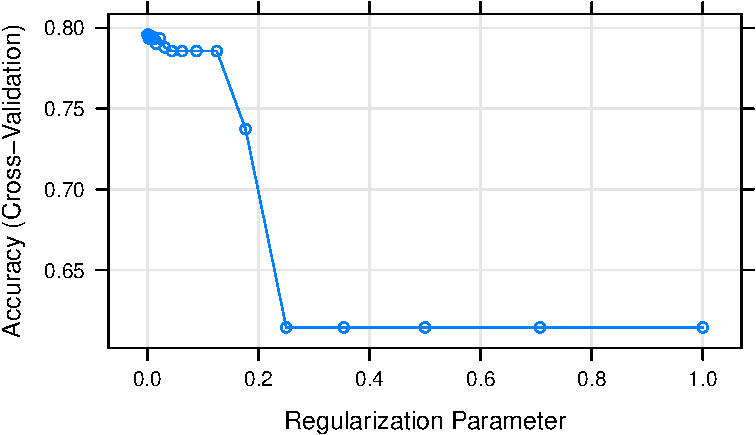
\includegraphics{index_files/figure-pdf/unnamed-chunk-17-1.pdf}

}

\end{figure}

\begin{center}\rule{0.5\linewidth}{0.5pt}\end{center}

\begin{Shaded}
\begin{Highlighting}[]
\CommentTok{\# Finding the optimal value for lambda}
\NormalTok{lambda\_optimal }\OtherTok{\textless{}{-}}\NormalTok{ lasso\_fit}\SpecialCharTok{$}\NormalTok{results}\SpecialCharTok{$}\NormalTok{lambda[}\FunctionTok{which.max}\NormalTok{(lasso\_fit}\SpecialCharTok{$}\NormalTok{results}\SpecialCharTok{$}\NormalTok{Accuracy)]}

\NormalTok{accuracy\_optimal }\OtherTok{\textless{}{-}} \FunctionTok{max}\NormalTok{(lasso\_fit}\SpecialCharTok{$}\NormalTok{results}\SpecialCharTok{$}\NormalTok{Accuracy)}

\FunctionTok{cat}\NormalTok{(}\StringTok{"The optimal value for lambda is"}\NormalTok{, lambda\_optimal, }\StringTok{"}\SpecialCharTok{\textbackslash{}n}\StringTok{"}\NormalTok{)}
\end{Highlighting}
\end{Shaded}

\begin{verbatim}
The optimal value for lambda is 9.536743e-07 
\end{verbatim}

\begin{Shaded}
\begin{Highlighting}[]
\FunctionTok{cat}\NormalTok{(}\StringTok{"The cross{-}validation accuracy for the optimal lambda is "}\NormalTok{, accuracy\_optimal, }\StringTok{"}\SpecialCharTok{\textbackslash{}n}\StringTok{"}\NormalTok{)}
\end{Highlighting}
\end{Shaded}

\begin{verbatim}
The cross-validation accuracy for the optimal lambda is  0.7958675 
\end{verbatim}

\begin{Shaded}
\begin{Highlighting}[]
\NormalTok{lasso\_predictions }\OtherTok{\textless{}{-}} \FunctionTok{predict}\NormalTok{(lasso\_fit)}
\NormalTok{lasso\_overview }\OtherTok{\textless{}{-}} \FunctionTok{overview}\NormalTok{(lasso\_predictions, df}\SpecialCharTok{$}\NormalTok{y)}
\NormalTok{lasso\_overview}
\end{Highlighting}
\end{Shaded}

\begin{verbatim}
  accuracy    error false_positive_rate false_negative_rate
1 0.800451 0.199549            0.133945           0.3040936
\end{verbatim}

3.5 (25 points)

First, use the \texttt{model.matrix()} function to convert the
covariates of \texttt{df} to a matrix format

\begin{Shaded}
\begin{Highlighting}[]
\NormalTok{covariate\_matrix }\OtherTok{\textless{}{-}} \FunctionTok{model.matrix}\NormalTok{(full\_model)[, }\SpecialCharTok{{-}}\DecValTok{1}\NormalTok{]}
\end{Highlighting}
\end{Shaded}

Now, initialize the covariates \(X\) and the response \(y\) as
\texttt{torch} tensors

\begin{Shaded}
\begin{Highlighting}[]
\NormalTok{X }\OtherTok{\textless{}{-}} \FunctionTok{torch\_tensor}\NormalTok{(covariate\_matrix, }\AttributeTok{dtype =} \FunctionTok{torch\_float}\NormalTok{())}
\NormalTok{y }\OtherTok{\textless{}{-}} \FunctionTok{torch\_tensor}\NormalTok{(df}\SpecialCharTok{$}\NormalTok{y, }\AttributeTok{dtype =} \FunctionTok{torch\_float}\NormalTok{())}
\end{Highlighting}
\end{Shaded}

Using the \texttt{torch} library, initialize an \texttt{nn\_module}
which performs logistic regression for this dataset. (Remember that we
have 6 different covariates)

\begin{Shaded}
\begin{Highlighting}[]
\NormalTok{logistic }\OtherTok{\textless{}{-}} \FunctionTok{nn\_module}\NormalTok{(}
  \AttributeTok{initialize =} \ControlFlowTok{function}\NormalTok{() \{}
\NormalTok{    self}\SpecialCharTok{$}\NormalTok{f }\OtherTok{\textless{}{-}} \FunctionTok{nn\_linear}\NormalTok{(}\DecValTok{6}\NormalTok{,}\DecValTok{1}\NormalTok{)}
\NormalTok{    self}\SpecialCharTok{$}\NormalTok{g }\OtherTok{\textless{}{-}} \FunctionTok{nn\_sigmoid}\NormalTok{()}
\NormalTok{  \},}
  \AttributeTok{forward =} \ControlFlowTok{function}\NormalTok{(x) \{}
\NormalTok{    x }\SpecialCharTok{\%\textgreater{}\%}
\NormalTok{    self}\SpecialCharTok{$}\FunctionTok{f}\NormalTok{() }\SpecialCharTok{\%\textgreater{}\%}
\NormalTok{    self}\SpecialCharTok{$}\FunctionTok{g}\NormalTok{()}
\NormalTok{  \}}
\NormalTok{)}

\NormalTok{f }\OtherTok{\textless{}{-}} \FunctionTok{logistic}\NormalTok{()}
\end{Highlighting}
\end{Shaded}

You can verify that your code is right by checking that the output to
the following code is a vector of probabilities:

\begin{Shaded}
\begin{Highlighting}[]
\FunctionTok{f}\NormalTok{(X)}
\end{Highlighting}
\end{Shaded}

\begin{verbatim}
torch_tensor
 0.2402
 0.9827
 0.1258
 0.9019
 0.0522
 0.1339
 0.4057
 0.9560
 0.0799
 0.9035
 0.8433
 0.0171
 0.2579
 0.0938
 0.3839
 0.0087
 0.9866
 0.2607
 0.2513
 0.1778
 0.2789
 0.0837
 0.3601
 0.6986
 0.9014
 0.0944
 0.1309
 1.0000
 0.1547
 0.1910
... [the output was truncated (use n=-1 to disable)]
[ CPUFloatType{887,1} ][ grad_fn = <SigmoidBackward0> ]
\end{verbatim}

Now, define the loss function \texttt{Loss()} which takes in two tensors
\texttt{X} and \texttt{y} and a function \texttt{Fun}, and outputs the
\textbf{Binary cross Entropy loss} between \texttt{Fun(X)} and
\texttt{y}.

\begin{Shaded}
\begin{Highlighting}[]
\NormalTok{Loss }\OtherTok{\textless{}{-}} \ControlFlowTok{function}\NormalTok{(X, y, Fun)\{}
  \FunctionTok{nn\_bce\_loss}\NormalTok{()(}\FunctionTok{Fun}\NormalTok{(X), y)}
\NormalTok{\}}
\end{Highlighting}
\end{Shaded}

Initialize an optimizer using \texttt{optim\_adam()} and perform
\(n=1000\) steps of gradient descent in order to fit logistic regression
using \texttt{torch}.

\begin{Shaded}
\begin{Highlighting}[]
\NormalTok{f }\OtherTok{\textless{}{-}} \FunctionTok{logistic}\NormalTok{()}
\NormalTok{optimizer }\OtherTok{\textless{}{-}} \FunctionTok{optim\_adam}\NormalTok{(f}\SpecialCharTok{$}\NormalTok{parameters, }\AttributeTok{lr=}\FloatTok{0.01}\NormalTok{) }\CommentTok{\# Insert your code here}

\NormalTok{n }\OtherTok{\textless{}{-}} \DecValTok{1000}
\ControlFlowTok{for}\NormalTok{ (i }\ControlFlowTok{in} \DecValTok{1}\SpecialCharTok{:}\NormalTok{n)\{}
\NormalTok{    loss }\OtherTok{\textless{}{-}} \FunctionTok{Loss}\NormalTok{(X, y, f)}
    
\NormalTok{    optimizer}\SpecialCharTok{$}\FunctionTok{zero\_grad}\NormalTok{()}
\NormalTok{    loss}\SpecialCharTok{$}\FunctionTok{backward}\NormalTok{()}
\NormalTok{    optimizer}\SpecialCharTok{$}\FunctionTok{step}\NormalTok{()}
    
    \ControlFlowTok{if}\NormalTok{ (i }\SpecialCharTok{\%\%} \DecValTok{100} \SpecialCharTok{==} \DecValTok{0}\NormalTok{) \{}
        \FunctionTok{cat}\NormalTok{(}\FunctionTok{sprintf}\NormalTok{(}\StringTok{"Step \%d, Loss: \%.4f}\SpecialCharTok{\textbackslash{}n}\StringTok{"}\NormalTok{, i, loss))}
\NormalTok{    \}}
\NormalTok{\}}
\end{Highlighting}
\end{Shaded}

\begin{verbatim}
Step 100, Loss: -36.3340
Step 200, Loss: -37.6889
Step 300, Loss: -38.0761
Step 400, Loss: -38.2684
Step 500, Loss: -38.3647
Step 600, Loss: -38.3652
Step 700, Loss: -38.4606
Step 800, Loss: -38.4609
Step 900, Loss: -38.4614
Step 1000, Loss: -38.4622
\end{verbatim}

Using the final, optimized parameters of \texttt{f}, compute the compute
the predicted results on \texttt{X}

\begin{Shaded}
\begin{Highlighting}[]
\NormalTok{predicted\_probabilities }\OtherTok{\textless{}{-}} \FunctionTok{f}\NormalTok{(X) }\SpecialCharTok{\%\textgreater{}\%} \FunctionTok{as\_array}\NormalTok{()}
\NormalTok{torch\_predictions }\OtherTok{\textless{}{-}} \FunctionTok{ifelse}\NormalTok{(predicted\_probabilities }\SpecialCharTok{\textgreater{}=} \FloatTok{0.5}\NormalTok{, }\DecValTok{1}\NormalTok{, }\DecValTok{0}\NormalTok{)}

\NormalTok{torch\_overview }\OtherTok{\textless{}{-}} \FunctionTok{overview}\NormalTok{(torch\_predictions, df}\SpecialCharTok{$}\NormalTok{y)}
\NormalTok{torch\_overview}
\end{Highlighting}
\end{Shaded}

\begin{verbatim}
   accuracy     error false_positive_rate false_negative_rate
1 0.3855693 0.6144307                   1                   0
\end{verbatim}

\begin{center}\rule{0.5\linewidth}{0.5pt}\end{center}

3.6 (5 points)

Create a summary table of the \texttt{overview()} summary statistics for
each of the \(4\) models we have looked at in this assignment, and
comment on their relative strengths and drawbacks.

\begin{Shaded}
\begin{Highlighting}[]
\NormalTok{combine\_overview }\OtherTok{\textless{}{-}} \FunctionTok{rbind}\NormalTok{(full\_model\_overview, stepwise\_overview, lasso\_overview, torch\_overview) }\SpecialCharTok{\%\textgreater{}\%}
  \FunctionTok{mutate}\NormalTok{(}\AttributeTok{Model =} \FunctionTok{c}\NormalTok{(}\StringTok{\textquotesingle{}Full Model\textquotesingle{}}\NormalTok{, }\StringTok{\textquotesingle{}Stepwise Regression\textquotesingle{}}\NormalTok{, }\StringTok{\textquotesingle{}LASSO\textquotesingle{}}\NormalTok{, }\StringTok{\textquotesingle{}Torch\textquotesingle{}}\NormalTok{))}
  
\NormalTok{combine\_overview }\OtherTok{\textless{}{-}}\NormalTok{ combine\_overview[, }\FunctionTok{c}\NormalTok{(}\StringTok{\textquotesingle{}Model\textquotesingle{}}\NormalTok{, }\StringTok{\textquotesingle{}accuracy\textquotesingle{}}\NormalTok{, }\StringTok{\textquotesingle{}error\textquotesingle{}}\NormalTok{, }\StringTok{\textquotesingle{}false\_positive\_rate\textquotesingle{}}\NormalTok{, }\StringTok{\textquotesingle{}false\_negative\_rate\textquotesingle{}}\NormalTok{)]}

\NormalTok{combine\_overview}
\end{Highlighting}
\end{Shaded}

\begin{verbatim}
                Model  accuracy     error false_positive_rate
1          Full Model 0.0000000 1.0000000                 NaN
2 Stepwise Regression 0.8049605 0.1950395            0.133945
3               LASSO 0.8004510 0.1995490            0.133945
4               Torch 0.3855693 0.6144307            1.000000
  false_negative_rate
1                 NaN
2           0.2923977
3           0.3040936
4           0.0000000
\end{verbatim}

\begin{quote}
Based on the output, we can see that the Stepwise Regression model seems
to performs slightly better than LASSO model, and far better than the
remaining two models. LASSO model selects a smaller set of predictors
and has a lower false positive rate. The Full model performs poorly and
hence is not suitable for the data given. However, it is imperative to
note that the relative strengths and weaknesses of the models may depend
on the specific context and the goals of the analysis.
\end{quote}

\pagebreak

---

\begin{tcolorbox}[enhanced jigsaw, breakable, colframe=quarto-callout-note-color-frame, bottomtitle=1mm, leftrule=.75mm, bottomrule=.15mm, arc=.35mm, titlerule=0mm, coltitle=black, colback=white, colbacktitle=quarto-callout-note-color!10!white, opacitybacktitle=0.6, toptitle=1mm, opacityback=0, title=\textcolor{quarto-callout-note-color}{\faInfo}\hspace{0.5em}{Session Information}, toprule=.15mm, left=2mm, rightrule=.15mm]

Print your \texttt{R} session information using the following command

\begin{Shaded}
\begin{Highlighting}[]
\FunctionTok{sessionInfo}\NormalTok{()}
\end{Highlighting}
\end{Shaded}

\begin{verbatim}
R version 4.2.2 (2022-10-31)
Platform: x86_64-apple-darwin17.0 (64-bit)
Running under: macOS Big Sur ... 10.16

Matrix products: default
BLAS:   /Library/Frameworks/R.framework/Versions/4.2/Resources/lib/libRblas.0.dylib
LAPACK: /Library/Frameworks/R.framework/Versions/4.2/Resources/lib/libRlapack.dylib

locale:
[1] en_US.UTF-8/en_US.UTF-8/en_US.UTF-8/C/en_US.UTF-8/en_US.UTF-8

attached base packages:
[1] stats     graphics  grDevices datasets  utils     methods   base     

other attached packages:
 [1] numDeriv_2016.8-1.1 broom_1.0.4         nnet_7.3-18        
 [4] torch_0.9.1         caret_6.0-94        lattice_0.20-45    
 [7] ggplot2_3.4.1       car_3.1-2           carData_3.0-5      
[10] corrplot_0.92       stringr_1.5.0       purrr_1.0.1        
[13] tidyr_1.3.0         readr_2.1.4         dplyr_1.1.1        

loaded via a namespace (and not attached):
 [1] nlme_3.1-160         lubridate_1.9.2      bit64_4.0.5         
 [4] tools_4.2.2          backports_1.4.1      utf8_1.2.3          
 [7] R6_2.5.1             rpart_4.1.19         colorspace_2.1-0    
[10] withr_2.5.0          tidyselect_1.2.0     processx_3.8.0      
[13] bit_4.0.5            compiler_4.2.2       glmnet_4.1-7        
[16] cli_3.6.1            labeling_0.4.2       scales_1.2.1        
[19] proxy_0.4-27         callr_3.7.3          digest_0.6.31       
[22] rmarkdown_2.21       coro_1.0.3           pkgconfig_2.0.3     
[25] htmltools_0.5.5      parallelly_1.35.0    fastmap_1.1.1       
[28] rlang_1.1.0          shape_1.4.6          generics_0.1.3      
[31] farver_2.1.1         jsonlite_1.8.4       ModelMetrics_1.2.2.2
[34] magrittr_2.0.3       Matrix_1.5-1         Rcpp_1.0.10         
[37] munsell_0.5.0        fansi_1.0.4          abind_1.4-5         
[40] lifecycle_1.0.3      stringi_1.7.12       pROC_1.18.0         
[43] yaml_2.3.7           MASS_7.3-58.1        plyr_1.8.8          
[46] recipes_1.0.5        grid_4.2.2           parallel_4.2.2      
[49] listenv_0.9.0        splines_4.2.2        hms_1.1.3           
[52] knitr_1.42           ps_1.7.3             pillar_1.9.0        
[55] future.apply_1.10.0  reshape2_1.4.4       codetools_0.2-18    
[58] stats4_4.2.2         glue_1.6.2           evaluate_0.20       
[61] data.table_1.14.8    renv_0.16.0-53       vctrs_0.6.1         
[64] tzdb_0.3.0           foreach_1.5.2        gtable_0.3.3        
[67] future_1.32.0        xfun_0.38            gower_1.0.1         
[70] prodlim_2019.11.13   e1071_1.7-13         class_7.3-20        
[73] survival_3.4-0       timeDate_4022.108    tibble_3.2.1        
[76] iterators_1.0.14     hardhat_1.3.0        lava_1.7.2.1        
[79] timechange_0.2.0     globals_0.16.2       ipred_0.9-14        
\end{verbatim}

\end{tcolorbox}



\end{document}
